% Drawing 144/04-7 -- folder 144, batch 04, archive page 77 (PDF page 78).
% Transcription: En bas à gauche, une sphère au crayon : l'équateur tracé en ellipse, avec des points marqués dessus (le polygone $P$ plongé sur un grand cercle).
% Kind: sphere with the polygon P on a great circle. Method 2 (schematic redraw from the facsimile). Status: ok.
% Notes: Pencil sphere; the equator drawn as an elongated ellipse, overinked, with marked points on it. The dense marginal writing to the left (on the slanted text block) is not drawn.
% Coordinates: 1 unit = 1 mm = 1/100 of the crop width (bbox in page fractions: [0.13, 0.76, 0.35, 0.86]).
% Redrawn by Claude (claude-opus-5-5), issue #73, 2026-11-07; not checked by a human; not compiled (no TeX in the session).
% Rights: reproduces part of the work -- behind RENDER_TRANSCRIPTS, never published by itself.
\documentclass[tikz,border=3pt]{standalone}
\usepackage{amsmath,amssymb}
\usetikzlibrary{patterns,arrows.meta}
\tikzset{pencil/.style={black!45}, struck/.style={black!35}, mark/.style={circle,draw,inner sep=1.3pt}, pt/.style={circle,fill,inner sep=0.9pt}, opt/.style={circle,draw,fill=white,inner sep=1.1pt}}
\begin{document}
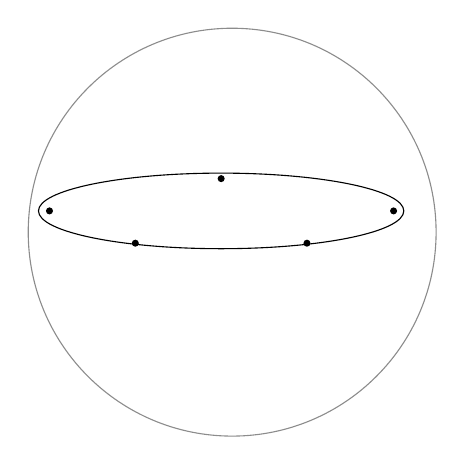
\begin{tikzpicture}[x=1mm,y=1mm,line cap=round,line join=round,font=\scriptsize]
\draw[pencil] (40,-36.8) circle[radius=25.9];
\draw (38.6,-34.1) ellipse[x radius=23.2, y radius=4.8];
\node[pt] at (16.8,-34.1) {};
\node[pt] at (38.6,-30) {};
\node[pt] at (60.5,-34.1) {};
\node[pt] at (27.7,-38.2) {};
\node[pt] at (49.5,-38.2) {};
\end{tikzpicture}
\end{document}
